\hypertarget{ht__move_8c}{
\section{ht\_\-move.c File Reference}
\label{ht__move_8c}\index{ht_move.c@{ht\_\-move.c}}
}


\subsection{Detailed Description}
\begin{Desc}
\item[For internal use only.]
This file contains the implementation of the \hyperlink{group__dbprim__hash_ga12}{ht\_\-move()} function, used to move a hash table entry to correspond to a new key.\end{Desc}


Definition in file \hyperlink{ht__move_8c-source}{ht\_\-move.c}.

{\tt \#include \char`\"{}dbprim.h\char`\"{}}\par
{\tt \#include \char`\"{}dbprim\_\-int.h\char`\"{}}\par


Include dependency graph for ht\_\-move.c:\begin{figure}[H]
\begin{center}
\leavevmode
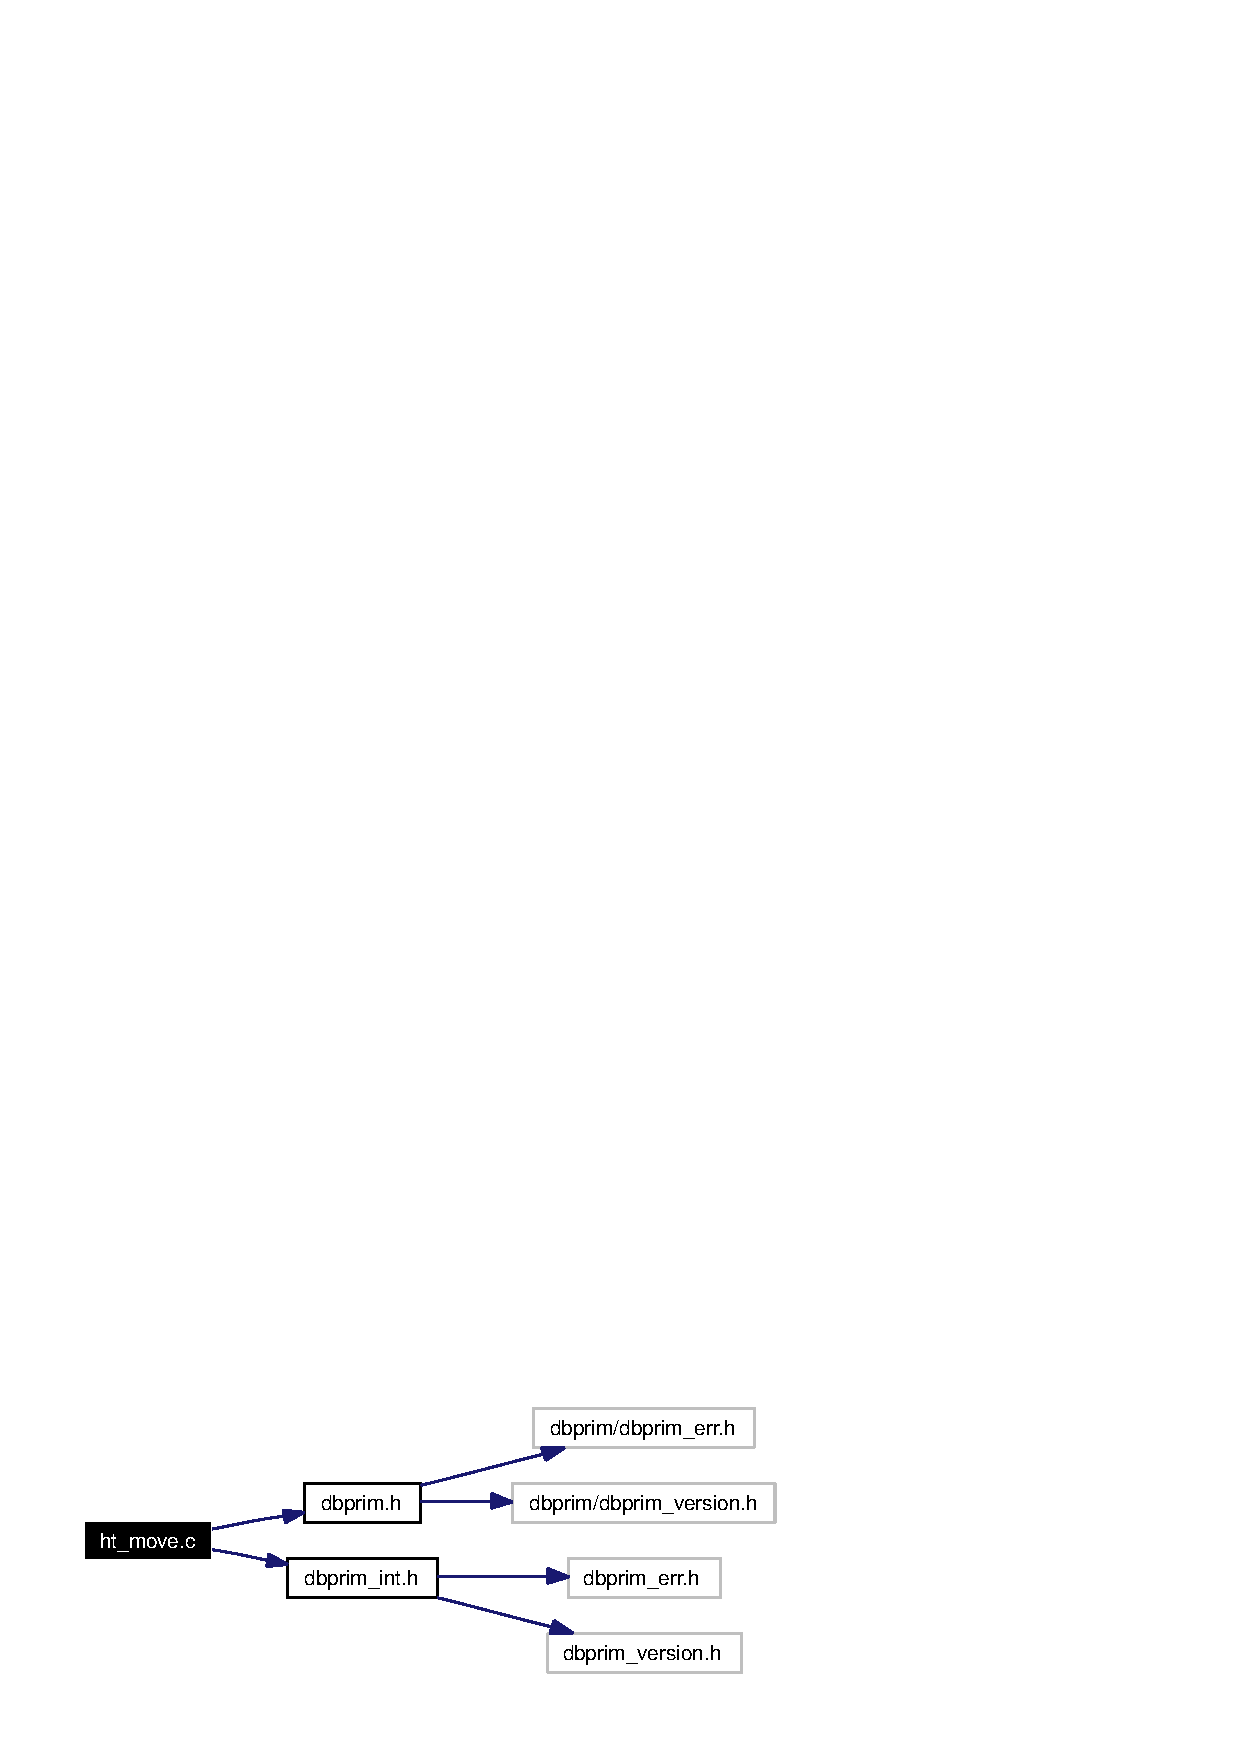
\includegraphics[width=188pt]{ht__move_8c__incl}
\end{center}
\end{figure}
\subsection*{Functions}
\begin{CompactItemize}
\item 
unsigned long \hyperlink{group__dbprim__hash_ga12}{ht\_\-move} (\hyperlink{struct__hash__table__s}{hash\_\-table\_\-t} $\ast$table, \hyperlink{struct__hash__entry__s}{hash\_\-entry\_\-t} $\ast$entry, \hyperlink{struct__db__key__s}{db\_\-key\_\-t} $\ast$key)
\begin{CompactList}\small\item\em Move an entry in the hash table. \item\end{CompactList}\end{CompactItemize}
